Lepton universality is one of the cornerstones of the Standard Model of particle physics. 
In the past years interesting hints of lepton non-universality have been seen in semi-leptonic decays of B hadrons~\cite{HFLAV16} where an excess of $\tau$ final states over $e,\mu$ final states is seen at the level of 4 standard deviations.
Measurements from LEP on W decays also show a hint of non universality at the level of a few percent~\cite{LEP-2}, again with a surplus of $\tau$ final states: 
\begin{equation}
  \label{eq:LEP_BRoverBRAll}
  \frac{2BR(W\to\tau\nu)}{BR(W\to\mu\nu)+BR(W\to e\nu)} = 1.077 \pm 0.026
\end{equation}
resulting in a poor agreement at the level of 2.8 standard deviations, with all correlations included.

Both results are shown in Figure~\ref{fig:lnuhints}.

\begin{figure}[htbp]
\centering
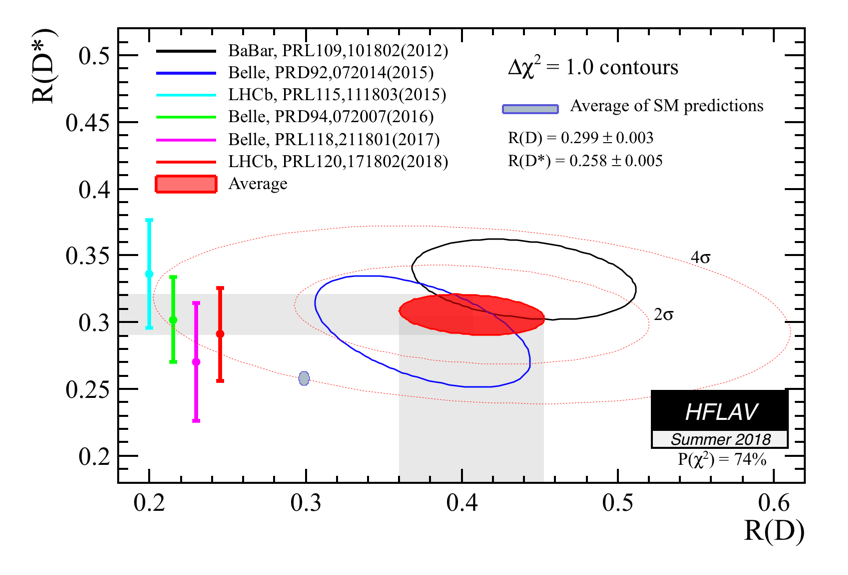
\includegraphics[width=10cm]{figures/01_intro/rdrds_summer18.png}
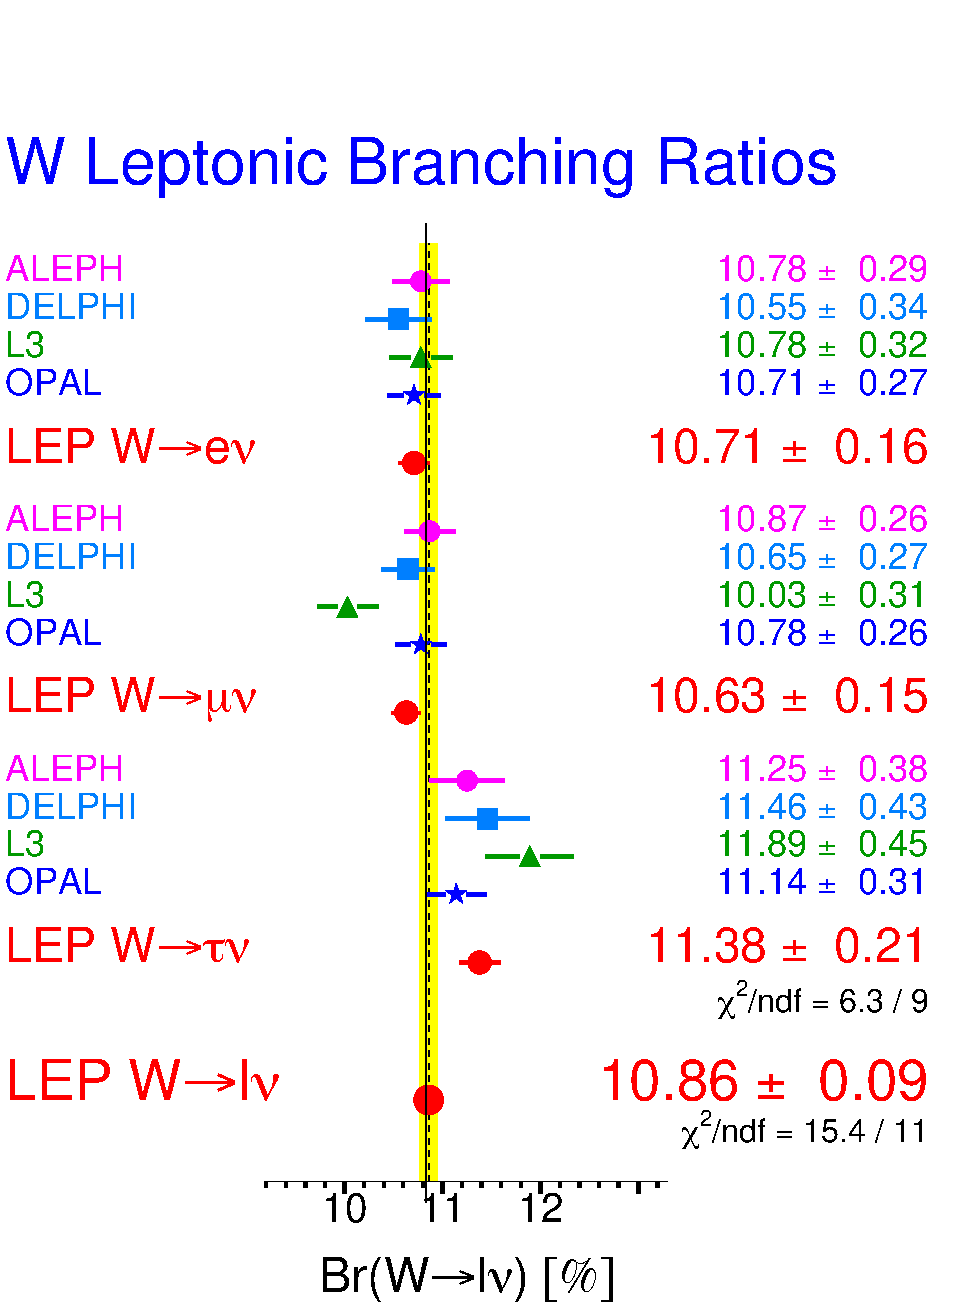
\includegraphics[width=6cm]{figures/01_intro/4f_brlv_lep_2008.pdf}
\caption{Left: Lepton universality in $B\to D^{(*)}$ decay from \cite{HFLAV16}. 
Right:  W leptonic branching ratios from \cite{LEP-2}}
\label{fig:lnuhints}
\end{figure}


\subsection{Summary of the Analysis Strategy}

The ATLAS experiment has produced over $10^9$ W decays to leptons, which allows us to make a high-precision measurement of lepton (non)-universality in prompt W decay by measuring the ratio $R_{\tau/\mu} =  BR (W\to \tau\nu \to \ell\nu\bar{\nu}) / BR (W \to \ell\nu)$, where $\ell = e, \mu$,  in which many of the systematic effects related to lepton identification cancel. 
Most leptons comes from prompt $W$ decay since the branching fraction of $\tau$ to leptons is 17.39 \% and many leptons coming from $W\to\tau\to \ell$ decay do not make it through the L1 trigger because of their lower momentum. 
Our first step is identification of the parts of the phase space enriched in $\tau$ decays using a multivariate classifier based on kinematic information and on the impact parameter of the lepton $d_0$.
Since these two variables are largely uncorrelated we can constrain the efficiency from data.

Same way as it is described in Top group analysis paper \cite{Mcfayden:2667199}, this analysis is setup to measure the ratio of the parameter of interest $R(\tau/\mu)$ in data and MC:
\begin{equation}
  \label{eq:fit_poi}
  \mu_{R(\tau/\mu)} = R^{full}(\tau/\mu) = \frac{BR(W\to\tau\nu)}{BR(W\to\mu\nu)}
\end{equation}
But instead of measuring tag and prompt leptons, we are working with single lepton triggers. 
This leads us to one of the main analysis challenges: good control over single trigger related systematics.


Control regions are defined to constrain the modelling of the major backgrounds: $Z\to\ell\ell$ boson production and QCD fake leptons.
Additional $Z\to\tau\tau$ leptonic control region is get used for $d_0$ correction studies.

Similarly as it was done in \cite{Mcfayden:2667199}, we define next list of categories of leptons according to their truth origin:
\begin{itemize}
\item \textbf{prompt ($W$)} leptons are leptons produced in $W\to\ell\nu$ decays.
\item \textbf{tau} are leptons produced in the leptonic decay chain $W \to \tau\nu \to \ell\nu\bar{\nu}$.
\item \textbf{prompt (non-$W$)} are leptons from $Z^0$ or other EWK process where these leptons do not originate from $W$ decays: for example di-boson, single top or $t\bar{t}$ process.
\item \textbf{``fake''} are reconstructed leptons from all other sources, including wrongly identified leptons.
\end{itemize}

A two-dimensional fit is performed in BDT and $d_0$ of the lepton.
The overall rate of the $W$ events is allowed to float along with the property of interest -- the ratio of $W \to \tau\nu$ to $W \to \ell\nu$ events.
The combined $d_0$--$p_T$ fit allows the best separation between prompt-, tau- and fake leptons.

Initial studies are performed for both electron and muon $W$ decay channels, but we focus on the ratio to muons rather then electrons for this analysis due to the lower rate of bremsstrahlung of muons and lower fakes background contribution.